\section{Robotic Reinforcement Learning}

% ---------------------------------------------------------------- Thread transition
\begin{frame}{}
\vfill
\centering
{\large Thread 3 of 3}\\[0.5em]
{\LARGE \textbf{Robotics}}\\[0.8em]
{\footnotesize\itshape What breaks when the environment is \emph{physical}: sample cost, safety, resets, and the sim-to-real gap.}
\vfill
\end{frame}

% ================================================================ 5.1
% Why real-world robot RL is hard (two-column comparison, not TikZ)
\begin{frame}{Why Real-World Robot RL Is Hard}
\begin{columns}[T]
\begin{column}{0.48\textwidth}
\centering
\setlength{\fboxsep}{6pt}%
\colorbox{boxgreen!50}{\parbox{0.9\linewidth}{\centering\textbf{Simulation}}}\\[0.5em]
\footnotesize
\begin{itemize}\itemsep0.2em
    \item cheap; millions of steps
    \item parallelizable across machines
    \item failures are free
    \item \emph{but:} a \textbf{reality gap}
\end{itemize}
\end{column}
\begin{column}{0.48\textwidth}
\centering
\setlength{\fboxsep}{6pt}%
\colorbox{boxred!40}{\parbox{0.9\linewidth}{\centering\textbf{Real hardware}}}\\[0.5em]
\footnotesize
\begin{itemize}\itemsep0.2em
    \item expensive, slow, safety-critical
    \item \textbf{resets are a real problem} \scriptsize(who picks the object back up?)
    \item sparse / hard-to-engineer reward
\end{itemize}
\end{column}
\end{columns}
\vfill
\begin{center}
\setlength{\fboxsep}{6pt}%
\colorbox{boxblue!50}{\parbox{0.9\textwidth}{\centering\footnotesize
Four obstacles (\textbf{sample efficiency, safety, resets, reward
specification}) are why off-the-shelf RL does not transfer to hardware.}}
\end{center}
\end{frame}

% ================================================================ 5.2
% Sim-to-real & domain randomization (fallback schematic - no figure available)
\begin{frame}{Sim-to-Real: Domain Randomization}
\centering
\resizebox{0.94\linewidth}{!}{%
\begin{tikzpicture}[font=\footnotesize,
    sim/.style={draw, rounded corners, minimum width=3.2cm, minimum height=0.8cm, align=center, fill=boxblue},
    ar/.style={-{Stealth[length=2.2mm]}, thick}]
  \node[sim] (s1) at (0,1.6)  {sim: friction $a$, mass $a$, lighting $a$};
  \node[sim] (s2) at (0,0.4)  {sim: friction $b$, mass $b$, lighting $b$};
  \node[sim] (s3) at (0,-0.8) {sim: friction $c$, mass $c$, lighting $c$};
  \node[draw, rounded corners, fill=sysblue, minimum width=2.2cm, minimum height=1.0cm,
        align=center] (pol) at (5.2,0.4) {one\\policy $\pi_\theta$};
  \node[draw, rounded corners, fill=mlgreen, minimum width=2.4cm, minimum height=1.0cm,
        align=center] (real) at (9.4,0.4) {real robot\\(deploy)};
  \draw[ar] (s1.east) -- (pol.north west);
  \draw[ar] (s2.east) -- (pol.west);
  \draw[ar] (s3.east) -- (pol.south west);
  \draw[ar] (pol) -- (real);
\end{tikzpicture}%
}
\vfill
\begin{center}
\setlength{\fboxsep}{6pt}%
\colorbox{boxgreen!50}{\parbox{0.86\textwidth}{\centering\footnotesize
Train across a \emph{distribution} of randomized sims (friction, mass, latency,
textures, lighting) so the real world looks like just one more sample.}}
\end{center}
\vspace{0.3em}
{\footnotesize \textbf{Headline successes:} OpenAI Dactyl (in-hand cube, Akkaya
et al.\ 2019); legged locomotion (ANYmal, Hwangbo et al.\ 2019; massively
parallel sim, Rudin et al.\ 2022).}
\srcnote{\scriptsize Domain randomization: Tobin et al. \href{https://arxiv.org/abs/1703.06907}{Domain Randomization for Transferring Deep Neural Networks from Simulation to the Real World}, 2017.}
\end{frame}

% ================================================================ 5.3
% SERL (keep screenshots, add Day 6 SAC lineage)
\begin{frame}{Robotic RL in Practice: SERL}
\vfill
\centering
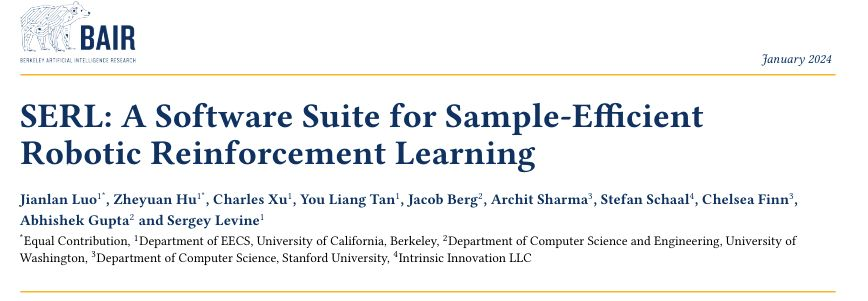
\includegraphics[width=0.9\linewidth,keepaspectratio]{images/rl-real-world/figures/serl-title.jpg}%
\srcnote{\scriptsize Luo et al. \href{https://serl-robot.github.io/}{SERL: A Software Suite for Sample-Efficient Robotic Reinforcement Learning}, 2024.}
\vfill
\end{frame}

\begin{frame}{SERL}
\begin{itemize}\itemsep0.4em
    \item A software framework for sample-efficient RL on real robots: an
          off-policy deep RL method plus tooling for computing rewards, resetting
          the environment, and a high-quality controller for a widely-adopted arm.
    \item \empr{Day 6 lineage:} \textbf{SERL $\leftarrow$ RLPD $\leftarrow$ SAC}, the same maximum-entropy method from Day 6, now learning on real
          hardware in \emph{minutes}.
\end{itemize}
\vfill
\centering
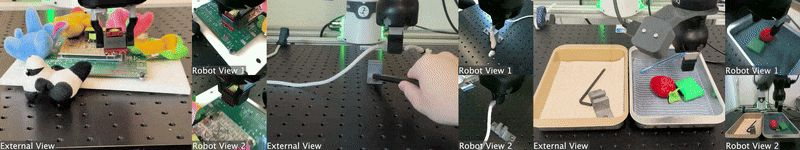
\includegraphics[width=0.92\linewidth,keepaspectratio]{images/rl-real-world/figures/robot-filmstrip.jpg}%
\srcnote{\scriptsize \href{https://github.com/rail-berkeley/serl}{github.com/rail-berkeley/serl}}
\end{frame}

\begin{frame}{SERL: Results}
\vfill
\centering
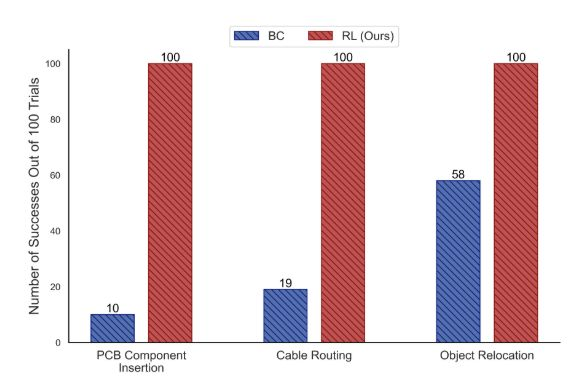
\includegraphics[width=0.6\linewidth,height=0.78\textheight,keepaspectratio]{images/rl-real-world/figures/robot-results.jpg}
\vfill
\end{frame}
